%\documentclass[a4paper,]{book}
\documentclass[a4paper, twoside,openright ,titlepage, 12pt]{book}
\usepackage[english]{babel}
\usepackage{preamble}
%\usepackage[MEK,60]{masterfrontpage}
%\setlength\parindent{0pt}

\begin{document}                                                                                                                          
%\maketitle
%\masterfrontpage
\pagenumbering{roman}
\tableofcontents
\newtheorem{theorem}{Theorem}[section]
\newtheorem{lemma}[theorem]{Lemma}
\pagenumbering{arabic}
%\chapter{A motivation for studying fluid-structure interaction}
The interaction between fluid and solids can be observed all around us in nature and has shown crucial in engineering. Examples in nature include swimming fish, flying birds, or trees bending in the wind. Man has learned from nature and has traditionally relied upon laboratory experiments to design windmills, aircrafts, and bridges. The importance of understanding fluid-structure (or solids) interaction (FSI) cannot be overstated, as the lack of such has demonstrated to be disastrous in the design of everything from bridges to airplanes. Let alone to emphasize our incapability to replicate the performance of nature; we're far away from designing a drone capable of flying like a hummingbird. However, laboratory experiments are inherently noisy, expensive, and results can be difficult to reproduce. A much cheaper and indeed smarter approach to studying FSI is using computers, or more specifically numerical simulations to gain fundamental insight to the interaction between fluids and solids. The latter has on the other hand shown to be difficult to realize, for a number of reasons related to both mathematical and computational reasons. Therefore, the goal of this thesis is to develop an open-source framework using standard techniques for solving FSI problems that can be used as a point of reference for future benchmarking of FEniCS-based FSI solvers. \\

The main goal of this thesis is to create a verified and validated monolithic fluid-structure interaction solver in FEniCS, which can handle large deformations. To achieve this, I have defined four subgoals: 

\begin{itemize}
\item Formulate a weak variation for a monolithic arbitrary Lagrangian Eulerian fluid-structure interaction problem.
\item Construct a finite element solver for the fluid-structure interaction problem.
\item Verify and validate a finite element solver for the fluid-structure interaction problem.
\item Compare the impact of discretization and mesh lifting operators on the final solution.
\item Improve computational efficiency of the implementation.
\end{itemize}


Each of the following subgoals will be addressed in separate chapters organized as follows: Balance of linear momentum for both solids and fluids are first introduced together with conservation of mass. The Eulerian, Lagrangian, and the arbitrary Lagrangian-Eulerian (ALE) frames of reference are briefly introduced to express the governing equations, before the equations describing FSI are derived. The numerical implementation is verified using the most rigorous convergence tests, before validation is performed against state-of-the-art benchmarks. Finally, computational speed-up is addressed together with long-term numerical stability of the coupled problem, and methods to overcome these challenges.
 

%\newpage
%\chapter{Governing equations}
%When studying the dynamics of a mediums with fluid or structure %properties under the influence of forces, we need in some sense a good description of how these forces act and alter the system itself.

Computational fluid-structure interaction is a multi-physics field of science, combining two separate fields of computational mechanics, computational fluid dynamics (CFD), and computational structure dynamics (CSM). While CFD and CSM traditionally have been considered as two distinct fields of science,  the goal of CFSI is to combine the separate fluid and structure problems ,and their interaction or \textit{coupling} to one another. Therefore, the study CFSI demands understanding of each separate field. This chapter presents the governing equations of the individual fluid and structure problem, and will form the basis for the next chapter.



\section{Continuum Mechanics}
To interpret nature, mathematical models are needed to describe how object around us reacts to external and/or internal stimuli. 
The mathematical models forms a basis for establishing elementary conservation laws and partial differential equations (PDE's), making scientist and egineers not only able to physical phenomena  in nature, but also predict them. Within mechanics, the response of materials undergoing applied forces or external stimuli is a primary interest. 
Fluid and solids are both materials built up by a sequence of atoms, meaning on a microscopic level, an observer will locate discontinuties and space within the material. Evaluating each atom, or \textit{material point}, is not impossible from a mathematical point of view. However, for mathematical moddeling and applications, the evaluation of each material point remains unpractical. In \textit{Continuum mechanics} (first formulated by Augustin-Louis Cauchy \cite{Merodio2011}), the microscopic structure of materials are  ignored, instead  asuming that the given material of interest is \textit{continously distributed} within the

 A body in continuum mechanics is considered to be matter continuously distributed in space.  Hence, no attention is given to the microscopic (atomic) structure of real materials although non-classical generalized theories of continuum mechanics are able to deal with the mesoscopic structure of matter (i.e. defects, cracks, dispersive lengths, .

To study the influence of forces acting on a continuum, we need an accurate framework to describe the effects. By a continuum we define  to a volume $V(t) \subset \mathbb{R}^d \ d \in (2, 3)$ 
consiting of particles,  continiously distributed throughout its own volume. The initial configuration $V(t = t_0)$  is assumed to be stress free,  defined as the \textit{reference configuration}. A
. We let $V(t)$ for 
$t \geq t_0$ denote the \textit{current configuration}. \\ \\
Central for the coordinate systems introduced in this chapter is the concept of \textit{material} and \textit{spatial} points. \textit{Material} points are simply the points defining the material, moving with it as it undergoes movement. \textit{Spatial} points on the other hand is the relative measure of movement of the \textit{material} points. (Godt nok ??). This concept will be further explained throughout the chapter.

\subsection{The structure problem and agrangian coordinate system}
As some medium is act upon by forces, one of the main properties of interest is the deformation of the medium. Hence we want to know the relative position of some particle from its initial configuration. \\
Let \^{x} be a particle in the reference  $\ha{x} \in \ha{V}$. 
Further let x(\^x, t) be the new location of a particle \^x for some time t such that $x \in V(t)$. We assume that no two particles $\ha{x}_a, \ha{x}_b \in \ha{V}$ occupy the same location for some time $V(t)$.
Then the transformation $\ha{T}(\ha{x}, t) = x(\ha{x}, t)$ maps a particle \ha{x} from the \textit{reference configuration} $\ha{V}$ to the  \textit{current configuration} $V(t)$
Assuming that the path for some \^{x} is continuous in time, we can define the inverse mapping $\ha{T}^{-1}(x, t) = \ha{x}(x, t)$, which maps $x(\ha{x}, t)$ back to its initial location at time $t = t_0$. \\
These mappings lets us track each particle from some \textit{reference configuration} to some deformed state at time t. 
Such a description of tracking each particle $\ha{x} \in \ha{V}$ is often denoted the \textit{Lagrangian Framework} and is a natural choice of describing structure mechanics. 

We define the \textit{deformation} 
\begin{align}
\ha{T}(\ha{x}, t) = \hat{u}(\ha{x},t) = x(\ha{x},t) - \ha{x} 
\end{align}

and the \textit{deformation velocity}
\begin{align}
\pder{\ha{T}(\ha{x}, t)}{t} = \hat{v}(\ha{x},t) = d_t x(\ha{x},t) = d_t \hat{u}(\ha{x},t) 
\end{align}

When tracking each particle as it moves, the \textit{material} and \textit{spatial} points coincide

\subsection{Eulerian coordinate system}
Considering a flow of fluid particles in a river, a \textit{Lagrangian} description of the particles would be tidious as the number of particles entring and leaving the domain quickly rise to a immense number. 
Instead consider defining a view-point $V$ fixed in time, and monitor every fluid particle passing the coordinate $x \in V(t)$ as time elapses. Such a description is defined as the \textit{Eulerian framework.} 
Therefore the Eulerian formulation is natural for describing fluid dynamics. \\
We can describe the particles occupying the \textit{current configuration} $V(t)$ for some time $t \geq t_0$ 
\begin{align*}
x = \ha{x} + \hat{u}(\ha{x}, t)	
\end{align*}
Since our domain is fixed we can define the deformation for a particle 
occupying position $x = x(\ha{x},t)$ as
\begin{align*}
\textbf{u}(x, t) = \hat{u}(\ha{x}, t) = x - \ha{x}	\\
\end{align*}
and its velocity
\begin{align*}
\textbf{v}(x,t) = \partial_t u(x,t) = \partial_t \hat{u}(\ha{x},t) = \hat{v}(\ha{x},t)
\end{align*}

It is important to mention that the we are not interested in which particle is occupying a certain point in our domain, but only its properties. As such the \textit{material} and \textit{spatial} points doesn't coincide in the \textit{Eulerian formulation}


\section{Deformation gradients}
When studying continuum mechanics we observe continious mediums as they are deformed over time. These deformations
results in relative changes of positions due to external and internal forces acting.. These relative changes of postition is called
\textit{strain}, and is the primary property that causes \textit{stress} within a medium of interest \cite{Richter2016}. We define stress as the internal forces that particles within a continuous material exert on each other. \\

The equations of mechanics can be derived with respect to either a deformed or undeformend configuration of our medium of interest. The choice of refering our equations to the current or reference configuration is indifferent from a theoretical point of view. In practice however this choice can have a severe impact on our strategy of solution methods and physical of modelling.   \cite{Wriggers2006}. We will therefore define the strain measures for both configurations of our medium.  

\begin{defn}
Deformation gradient. 
\begin{align}
\hat{F} = I + \hat{\nabla} \hat{u} 
\end{align} 
\end{defn}

Mind that deformation gradient of $\hat{u}$ is which respect to the reference configuration. 
From the assumption that no two particles $\ha{x}_a, \ha{x}_b \in \ha{V}$ occupy the same location for some time $V(t)$, the presented transformation must be linear. As a consequence from the invertible matrix theorem found in linear algebra, the linear operator \textbf{F} cannot be a singuar.  
We define the  \textit{determinant of the deformation gradient} as \textit{J}, which denotes the local change of volume of our domain. 

\begin{defn}
Determinant of the deformation gradient
\begin{align}
J = det(\hat{F}) = det( I + \hat{\nabla} \hat{u} ) \neq 0
\end{align} 
\end{defn}


By the assumption that the medium can't be selfpenetrated, we must limit  J to be greater than 0 \cite{Wriggers2006}

\section{Measures of Strain and Stress}
The equations describing forces on our domain can be derived in accordinance with the current or reference configuration. With this in mind, different measures of strain can be derived with respect to which configuration we are interested in. We will here by \cite{Richter2016} show the most common measures of strain. We will first introduce the right \textit{Cauchy-Green} tensor \textbf{C}, which is one of the most used strain measures \cite{Wriggers2006}. \\ Uttrykk 1.3 fra Godboka, LAG TEGNING \\ 

Let $\ha{x}, \ha{y} \in \ha{V}$ be two points in our referemce configuration and let $\ha{a} = \ha{y} - \ha{x}$ denote the
length of the line bewtween these two points. As our domain undergoes deformation let 
$x = \ha{x} + \hat{u}( \ha{x} ) $ and $x = \ha{y} + \hat{u}( \ha{y} )  $ be the position of our points in the current configuration, and let $a = y - x$ be our new line segment. By \cite{Richter2016} we have by first order Taylor expansion

\begin{align*}
&y - x = \ha{y} + \hat{u}(\ha{y}) - \ha{x} - \hat{u}(\ha{x}) = \
\ha{y} - \ha{x} + \hat{\nabla}\ha{u}(\ha{x}) (\ha{y} - \ha{x}) 
+ \mathcal{O}(|\ha{y} - \ha{x} |^2) \\
&\frac{y - x}{|\ha{y} - \ha{x}|} = [I + \hat{\nabla}\hat{u}(\ha{x} ]  
\frac{\ha{y} - \ha{x}}{|\ha{y} - \ha{x}|} + \mathcal{O}(|\ha{y} - \ha{x} |) 
\end{align*}

This detour from \cite{Richter2016}  we have that 
\begin{align*}
&a = y - x = \hat{F}(\ha{x})\ha{a} +  \mathcal{O}(|\ha{a} |^2) \\
&|a| = \sqrt{ (\hat{F}\ha{a},\hat{F}\ha{a})+ \mathcal{O} (|\ha{a}^3|)  } = 
 \sqrt{ (\ha{a}^T, \hat{F}^T\hat{F}\ha{a})} + \mathcal{O} (|\ha{a}^2|)  
\end{align*}

We let $\ha{C} = \ha{F}^T \ha{F}$ denote the right \textit{Cauchy-Green tensor}.
By observation the Cauchy-Green tensor is not zero at the reference configuration 
\begin{align*}
\ha{C} =  \ha{F}^T \ha{F} = (I + \hat{\nabla} \ha{u})^T (I + \hat{\nabla} \ha{u}) = 1
\end{align*}

Hence it is convenient to introduce a tensor which is zero at the reference configuration. We define the \textit{Grenn-Lagrange strain tensor}, which arises from the squard rate of change of the linesegment \ha{a} and \textit{a}. By using the definition of the Cauchy-Green tensor we have the relation
\begin{align*}
&\frac{1}{2}(|a|^2 + |\ha{a}|^2) = \frac{1}{2}(\ha{a}^T\hat{C}\ha{a}
 -\ha{a}^T \ha{a} ) + \mathcal{O}(|\ha{a}^3| = 
 \ha{a}^T \big(\frac{1}{2} (\hat{F}^T \hat{F} - I) \big) \ha{a} 
 + \mathcal{O}(\ha{a}^3) \\
&\hat{E} = \frac{1}{2}(\hat{C} - I)
\end{align*}

Both the \textit{right Cauchy-Green tensor} $\hat{C}$ and the \textit{Green-Lagrange} $\hat{E}$ are refered to the Lagrangian coordinate system, hence the \textit{reference configuration}. \\
Using similar arguments (see \cite{Richter2016}, compsda) Eulerian counterparts of the Lagrangian stress tensors can be derived.

The \textit{left Cauchy-Green} strain tensor 
\begin{align*}
\mathbf{b} = \ha{F} \ha{F}^T = 
\end{align*}
and the \textit{Euler-Almansi} strain tensor
\begin{align*}
\mathbf{e} = \frac{1}{2} (I - \hat{F}^{-1}\hat{F}^{-T}) = \hat{F}^{-1}\hat{E}\hat{F}^{T}
\end{align*}

It is important to note that strain itself is nothing else than the measurement of line segments under deformation. Therefore strain alone is purely an observation, and it is not dependent on the material of interest. However one expects that a material undergoing strain, will give  forces within the material due to neighboring material interacting with one another. Therefore one derive materialspecific models to describe how a certain material will react to a certain amount of strain.\\
These strain measures are used to define models for \textit{stress}, which is responsible for the deformation in materials (cite holzapfel). The dimention of stress is force per unit area.

\section{Governing Equations}
The fully Fluid-structure interaction problem is based on equations of balance laws, with auxiliary kinematic, dynamic and material relations. In this section, assumptions regarding these relations will be described briefly. A deeper review of the full FSI problem will be considered in the next chapter. 

\subsection{The Fluid}
We will throughout this thesis consider in-compressible fluids described by Navier-Stokes equations. We define the fluid density as $\rho_f$ and fluid viscosity $\nu_f$ to be constant in time. Our phsyical unknowns
fluid velocity $v_f$ and pressure $p_f$ both live in the time-dependent fluid domain  $\hat{\Omega}_f(t)$, with an eulerian configuration. Together with the equations of momentum and continuum, the Navier-Stokes equation is defined as,

\begin{equat}
\textit{Navier-Stokes equation}
\begin{align}
&\rho \pder{\mathbf{v}_f}{t} + \rho \mathbf{v}_f \cdot \nabla \mathbf{v}_f =
\nabla \cdot \sigma + \rho \mathbf{f}_f \hspace{4mm} \text{in} \hspace{2mm} \Omega_f \\
&\nabla \cdot \mathbf{v}_f = 0 \hspace{4mm} \text{in} \hspace{2mm} \Omega_f 
\end{align} 
\end{equat}
where $\mathbf{f}_s$ is some body force. 
Assuming a newtonian fluid the \textit{Cauchy stress sensor} $\sigma$ takes the form \newline $\sigma = -p_f I + \mu_f (\nabla \mathbf{v}_f + (\nabla \mathbf{v}_f)^T$.

Additional appropriate boundary conditions are supplemented to the equation for a given problem. The first type of of boundary conditions are Dirichlet boundary conditions, 
\begin{align}
\mathbf{v}_f = \mathbf{v}_f^D 
\hspace{4mm} \text{on} \hspace{2mm} \Gamma_f^D \subset \partial \Omega_f 
\end{align}
The second type of boundary condition are Neumann boundary conditions
\begin{align}
\sigma_f \cdot \mathbf{n} = \mathbf{g} 
\hspace{4mm} \text{on} \hspace{2mm} \Gamma_f^N \subset \partial \Omega_f 
\end{align}

\newpage
\subsection{The solid}
The governing equations for the solid mechanics are given by the blalance law,
\begin{equat}
\textit{Solid momentum}
\begin{align}
\rho_s \pder{\mathbf{v}_s}{t} = \nabla \cdot \bat{T} + \rho_s \mathbf{f}_s
\hspace{4mm} \text{in} \hspace{2mm} \hat{\Omega}_s
\end{align}
\end{equat}
defined in a Lagrangian coordinate system, with respect to an initial reference configuration $\hat{\Omega}_s$. The structure configuration is given by the displacement $\bat{u}_s$, with the relation
 $\pder{\bat{v}}{t} = \bat{u}_s$ to the solid velocity. The density of the structure is given by $\rho_s$, and $\bat{f}_s$ express any exterior body forces acting. The tensor $\bat{T}$ denotes the first Piola-Kirchhoff stress tensor, with the relation $\bat{T}  = \bat{J} \sigma_s \bat{F}^{-T}$ to the cauchy stress tensor. By definition the cauchy stress tensor is symmetric, however the first Piola-Kirchhoff tensor does not exhibit this property. As constitute equations often assumes this behaviour of symmetry, the second Piola-Kirchhoff tensor $\bat{S}_s$ is convenient as it is symmetric.  It is given by the relation to the firt Piola-Kirchhoff stress tensor by, 
 
 \begin{align*}
 \bat{S}_s = \bat{F}^{-T} \bat{T} = \hat{J} \bat{F}^{-1} \sigma_s \bat{F}^{-T}
 \end{align*}
 
According to the material of interest, several material models exist to model the induced stress given by material deformation. Most famous is Hooke's law, describing a linear relation between strain and stress, limited to a small-deformation regime. As we may no longer be in the range of small-deformation approximation were a linear-elastic material can be used, a consitent way to describe large deformations is needed. As such, for describing large deformation it is widley common to use a stress-strain relation based of the introduced Green Lagrangian strain tensor $\bat{E}$ and the second Piola-Kirchhoff stress tensor $\bat{S}$ \cite{Razzaq2010}. Therefore the material is assumed to follow a hyperelastic model, specifically the Vernant-Kirchhoff(STVK) model. Though STVK can handle large deformations, it is limited of the calculation of large strain \cite{Razzaq2010}. However since the deformations considered in this thesis are small, it will remain our primary choice of strain-stress relation.  STVK describes materials of compressible nature,  but is should be mentioned that for large deformation models describing incompressible materials can be considered. Specially the Incompressible Neo-Hooke (INH) model is considered in several publications (see \cite{Wick2013}, \cite{Richter2010c}), sharing the same hyperelastic properties as the STVK model. As both models handles large deformations, the INH is superior compared to STVK in the sense that it is valid for large strains aswell \cite{Razzaq2010}. \newpage
The STVK is one of the simplest hyperelastic model, as it only extend the famous Hooke's law into a non-linear regime by,

\begin{align*}
\sigma_s = \frac{1}{\hat{J}} \bat{F}(\lambda_s(Tr(\bat{E}) I + 2 \mu \bat{E})\bat{F}^{-T} \hspace{4mm}
\bat{S}_s = \lambda_s(Tr(\bat{E}) I + 2 \mu \bat{E} \\
\bat{E} = \frac{1}{2}(\bat{C} - I ) \hspace{4mm} \bat{C} = \bat{F}\bat{F}^{-T}
\end{align*} 
 where $\bat{C}$ is the right Cauchy-Green strain tensor mention in the last subchapter. 
  
 The solid is often characterized by the Possion ratio and Young modulus. Lamè coefficients  $\lambda_s$ and $\mu_s$ are then given by the relation.

\begin{align*}
&E_y = \frac{ \mu_s ( \lambda_s + 2 \mu_s) }{ ( \lambda_s + \mu_s ) } 
\hspace{5mm} \nu_s = \frac{\lambda_s}{2(\lambda_s + \mu_s)} \\
&\lambda_s = \frac{\nu E_y}{(1 + \nu_s)(1 - 2\nu_s)} \hspace{4mm} \mu_s = \frac{E_y}{2(1 + \nu_s)} 
\end{align*}

Since the solid deformation is a quantity of interest a kinematic condition must be defined for the system of the form
\begin{align}
\pder{\mathbf{v}_s}{t} = \mathbf{u_s} \hspace{4mm} \text{in} \hspace{2mm} \Omega_s
\end{align} 
One might ask the motivation of such an approach as the Lagrangian system could let us define the problem 
\begin{align}
\rho_s \ppder{\mathbf{u}_s}{t} = \nabla \cdot \mathbf{T} + \rho_s \mathbf{f}_s
\hspace{4mm} \text{in} \hspace{2mm} \Omega_s
\end{align}
directly solving for the main quantity of interest namely deformation. However solving for $\mathbf{v}_s$ is more convenient, as it lets us handle constraints for the fluid-structure interaction problem easier. As for the fluid problem we define Dirichlet and Neumann boundary conditions on the form

\begin{align*}
\mathbf{v}_s = \mathbf{v}_s^D 
\hspace{4mm} \text{on} \hspace{2mm} \Gamma_s^D \subset \partial \Omega_s  \\
\sigma_s \cdot \mathbf{n} = \mathbf{g}  
\hspace{4mm} \text{on} \hspace{2mm} \Gamma_s^N \subset \partial \Omega_s 
\end{align*}




%\newpage
\chapter{Computational Fluid Structure Interaction}

The multi-disciplinary nature of computational fluid-structure interaction , involves addressing issues regarding computational fluid dynamics and computational structure dynamics. In general, CFD and CSM are individually well-studied, in terms of numerical solution strategies. CFSI adds another layer of complexity to the solution process, (1) the \textit{coupling} of the fluid and solid equations , (2) the tracking of \textit{interface} separating the fluid and solid domains. The coupling pose two new conditions at the interface absent from the original fluid and solid conditions, which is \textit{continuity of velocity} and \textit{continuity of stress} at the interface.

\begin{align}
\mathbf{v}_f = \mathbf{v}_s \\
\mathbf{\sigma}_f \cdot \mathbf{n} = \mathbf{\sigma}_s \cdot \mathbf{n}
\end{align}


The tracking of the interface is a issue, due to the different description of motion used in the fluid and solid problem. If the natural coordinate system are used for the fluid problem and solid problem, namely the eulerian and lagrangian description of motion, the domains doesn't match and the interface. Tracking the interface is aslo essential for fulfilling the interface boundary conditions. As such only one of the domains can be described in its natural coordinate system, while the other domain needs to be defined in some transformed coordinate system.   \\ 

Fluid-structure interaction problems are formally divided into the \textit{monolithic} and \textit{partitioned} frameworks.  In the monolithic framework, the fluid and solid equations together with interface conditions are solved simultaneously. The monolithic approach has the advantage of fullfilling the \textit{kinematic} (1.1) and \textit{dynamic}(1.2) interface conditions with high accuracy. The method is then said to be \textit{strongly coupled}. However, the complexity of solving all the equations simuntainiously and the strong coupling contributes to a stronger nonlinear behaviour of the whole system \cite{Wick}. The complexity also makes monolithic implementations \textit{ad hoc} and less modular, and the nonlinearity makes solution time slow.

In the \textit{partitioned} framework one solves the equations of fluid and structure subsequently. Sovling the fluid and solid problems individually is beneficial, in terms of the wide range of optimized solvers and solution strategies developed for each sub-problem. A major drawback is the methods ability to enfore the \textit{kinematic} (1.1) and \textit{dynamic}(1.2) conditions at each timestep. Therefore partitioned solution strategies are defined as  \textit{weakly} coupled. However, by sub-iterations between each sub-problem at each timestep, (1.1) and (1.2) can be enforced with high accuracy, at the cost of increased compuational time. For some applications, low-accuracy of the interface conditions are suffictient such as aeroelasticity \cite{Fernandez2009}. \\

Capturing the interface is matter of its own, regardless of the the monolithic and partitioned frameworks.
The scope of interface methods are divided into \textit{interface-tracking} and \textit{interface-capturing } methods.\cite{Frei2016}. In the \textit{Interface-tracking} method, the mesh moves to accommodate for the movement of the structure as it deformes the spatial domain occupied by the fluid. As such, the mesh itself "tracks" the fluid-structure interface as the domain undergoes deformation. Interface-capturing yields better control of mesh resolution near the interface, which in turn yeilds better control of this critical area in terms of enforcing the interface conditions.
However, moving the mesh-nodes pose potential problems for mesh-entanglements, restricting the possible extent of deformations.  

In \textit{interface-capturing} methods one distinguish the fluid and solid domains by some phase variable over a fixed mesh, not resolved by the mesh iteself. This approach is in general not limitied in terms of deformations, but suffers from reduced accuracy at the interface. \cite{Frei2016}. 

\begin{figure}[h!]
  \centering
    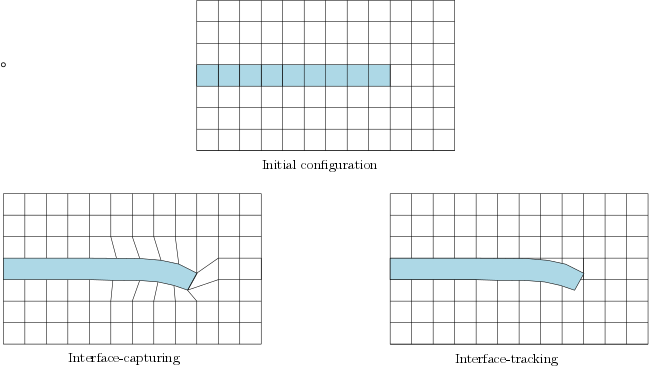
\includegraphics[scale=0.5]{./Fig/interface.png}
      \caption{Comparison of interface-tracking and interface-capturing for an elastic beam undergoing deformation}
\end{figure}

Among the multiple approaches within CFSI, the arbitary Lagrangia-Eulerian methos is chosen for this thesis. 



%We define $\Omega$ in the \textit{reference configuration} be partitioned in a fluid domain $\hat{\Omega_f}$ and a structure domain $\hat{\Omega_s}$ such that
%$\Omega = \hat{\Omega_f} \cup \hat{\Omega_s}$. Further we define the interface $\hat{\Gamma}$ as the interface between these domains such that $\Gamma_i = \hat{\partial \Omega_f} \cap \hat{\partial %\Omega_s}$. 
%The fluid-structure interaction problem is then defined by the fluid and solid equations, and the transmission of the \textit{kinematic} and \textit{dynamic} conditions on the interface $\hat{\Gamma}$. 


%\section{Fully Eulerian}
%This method keeps the fluid in its \textit{Eulerian coordinates}, and such can be seen as the natural counterpart of the ALE method \cite{Wick2013}. First proposed by , \cite{Dunne2006}. One motivation of such and approach is the handling of large-deformation, as the transformation to eulerian coordinates are purely natural.

\section{Arbitary Lagrangian Eulerian formulation}
The \textit{arbitary Lagrangian-Eulerian} formulation is the most popular approach within \textit{Interface-tracking} \cite{Richter2010a}, \cite{Frei2016}, initially developed to combine the strengths of the \textit{Lagranngian} and \textit{Eulerian} coordinate systems. In this approach the structure is given in its natural \textit{Lagrangian coordinate system}, while transforming the fluid domain into an artificial coordinate system similar to the \textit{Lagrangian coordinate system}. Since no natural displacement occur in the fluid domain, the transformation has no directly physical meaning \cite{Richter2010a}, \cite{Donea2004}. 
 
With this in mind, we will derive these transformations with the help of a new arbitary fixed reference system \ha{W}, following the ideas and approaches found in \cite{Richter2016}. Further we denote its deformation gradient as $\hat{F}_w$ and its determinant $\ha{J}_w$. Following the ideas from chapter 2, we introduce the invertibale mapping $\ha{T}_w : \ha{W} \rightarrow V(t)$ , with the scalar $\ha{f}(\ha{x}_W, t) = f(x,t) $ and vector $\hat{w}(\ha{x}_W, t) = \mathbf{w}(x,t) $ counterparts.\\ 
For $\ha{V} = \ha{W}$, $\ha{W}$ simply denotes the familiar Lagrangian description.
In the case $\ha{V} \neq \ha{W}$, $\ha{W}$ as pointed out earlier have no direct physical meaning.  Hence it is important to notice that the physical velocity $\hat{v}$ and the velocity of arbitrary domain $\pder{\ha{W}_w}{t}$ doesn't necessary coincide. This observation is essential, as we will soon see. \\

We will first define the transformation of spatial and temporal derivatives from $V(t)$ to $\ha{W}$ found in \cite{Richter2016}\\

\begin{lem}
Transformation of scalar spatial derivatives \\
\textit{Let f be a scalar function such that} $f: V(t) \rightarrow \mathbb{R}$, \textit{then} 
\begin{align}
\nabla f = \hat{F}_W^{-T} \hat{\nabla}\ha{f}
\end{align} 
\end{lem}

\begin{lem}
Transformation of vector spatial derivatives \\
\textit{Let \textbf{w} be a vector field such that} $\mathbf{w}: V(t) \rightarrow \mathbb{R}^d$, \textit{then} 
\begin{align}
\nabla \mathbf{w} = \hat{\nabla}\hat{w} \hat{F}_W^{-1} 
\end{align} 
\end{lem}

\begin{lem}
Transformation of scalar temporal derivatives \\
\textit{Let f be a scalar function such that} $f: V(t) \rightarrow \mathbb{R}$, \textit{then} 
\begin{align}
\pder{f}{t} = \pder{\ha{f} }{t} - (\hat{F}_W^{-1} \pder{\ha{T}_W}{t} \cdot \hat{\nabla}) \ha{f}
\end{align} 
\end{lem}

In addition we need a consistent way to transform the induced stresses in the \textit{Eulerian} coordinate system to $\ha{W}$. Hence we introduce the \textit{Piloa transformation}, found in most introduction courses in structure mechanics.
\\
\begin{lem}
T \\
\textit{Let \textbf{w} be a vector field such that} $\mathbf{w}: V(t) \rightarrow \mathbb{R}^d$, \textit{then the Piola transformation of w is defined by} 
\begin{align}
\mathbf{w} = \ha{J}_W \hat{F}^{-1}_W \hat{w}
\end{align} 
\end{lem}

The Piola transformation can be further extended to transform tensors, see \cite{Richter2016}, Orange book. This results is essential as it allows us to transform surface forces induced by the \textit{Cauchy stress tensor} on our arbitrary coordinate system $\ha{W}$. Lemma 1.4 brings us to \textit{the first Piola Kirchhoff stress tensor} $\hat{P} = \ha{J}_W \hat{\sigma}\hat{F}_W^{-T}$.

\subsection{ALE formulation of the fluid problem}

Recall the Navier-Stokes equation defined in the \textit{Eulerian coordinate system} V(t).
\begin{align*}
&\rho \pder{\mathbf{v}}{t} + \rho \mathbf{v} \cdot \nabla \mathbf{v} =
\nabla \cdot \sigma + \rho \mathbf{f} \\
&\nabla \cdot \mathbf{v} = 0
\end{align*}
Using our newly introduced transformations of derivatives we map the equation to the arbitrary reference system $\ha{W}$. We will first consider the transformation of the\textit{material derivative}. By 
\begin{align*}
\frac{d \mathbf{v}}{dt}(x,t) = \pder{\mathbf{v}}{t}(x,t) + \nabla \mathbf{v}(x,t) \cdot \pder{x}{t} \\
\frac{d \mathbf{v}}{dt}(x,t) = \pder{\mathbf{v}}{t}(x,t) + \nabla \mathbf{v}(x,t) \cdot \mathbf{v}
\end{align*}
Note $\pder{x}{t}$ is the velocity of particles and not the transformation velocity $\pder{\ha{T}_W}{t}$. By lemma(1.1, 1.2, 1.3) we have  

\begin{align*}
\frac{d \mathbf{v}}{dt}(x,t) = 
\pder{\hat{v}}{t}(x,t) - (\hat{F}_W^{-1}\pder{\ha{T}_W}{t} \cdot \hat{\nabla})\hat{v}
+ \hat{F}_W^{-T}\hat{\nabla}\hat{v} \cdot \hat{v} \\
\mathbf{v} \cdot \nabla \mathbf{v} = \nabla \mathbf{v} \mathbf{v} = 
\hat{\nabla}\hat{v}\hat{F}_W^{-1}\hat{v} = (\hat{F}_W^{-1}\hat{v} \cdot \hat{\nabla})\hat{v} \hspace{4mm} \textit{FINN KILDE}
\end{align*}

These results can be used to show that

\begin{align*}
\pder{\mathbf{v}}{t} + \mathbf{v} \cdot \nabla \mathbf{v} =
\pder{\hat{v}}{t} + (\hat{F}_W^{-1}(\hat{v} - \pder{\ha{T}_W}{t}) \cdot \hat{\nabla}) \hat{v}
\end{align*}

By applying \textit{the first Piola Kirchhoff stress tensor} directly we transform the surface stress by 

\begin{align*}
\nabla \cdot \sigma = \nabla \cdot (\ha{J}_W \hat{\sigma}\hat{F}_W^{-T})
\end{align*}
In general, $\sigma$ is presumed on the form of a Newtonian fluid.
However special care must be taken, as $\sigma \neq \hat{\sigma}$ due to spatial derivatives within the tensor. Hence 
\begin{align*}
\sigma = -p I + \mu_f(\nabla \mathbf{v} + (\nabla \mathbf{v})^T \\
\hat{\sigma} = -\ha{p} I + \mu_f(\hat{\nabla}\hat{v}\hat{F}_W^{-1} +\hat{F}_W^{-T}\hat{\nabla}\hat{v}^T )
\end{align*} 

For the conservation of continuum we apply the \textit{Piola Transformation} such that

\begin{align*}
\nabla \cdot \mathbf{v} = \nabla \cdot (\ha{J} \hat{F}_W^{-1} \hat{v})
\end{align*}

\subsection{ALE formulation of the solid problem}

With the introduced mapping identities we have the necessary tools to derive a full fluid-structure interaction problem defined of a fixed domain. Since the structure already is defined in its natural Lagrangian coordinate system, no further derivations are needed for defining the total problem.

\begin{equat}
\textit{ALE problem on a fixed domain}
\begin{align}
\ha{J} \pder{\hat{v}}{t} + \ha{J} (\hat{F}_W^{-1}(\hat{v} - \pder{\ha{T}_W}{t}) \cdot \hat{\nabla}) \hat{v}
= \nabla \cdot (\ha{J}_W \hat{\sigma}\hat{F}_W^{-T}) + \rho_f \ha{J} \mathbf{f}_f
\hspace{4mm} \text{in} \hspace{2mm} \Omega_f \\
\nabla \cdot (\ha{J} \hat{F}_W^{-1} \hat{v}) \hspace{4mm} \text{in} \hspace{2mm} \Omega_f \\
\rho_s \pder{\hat{v}_s}{t} = \nabla \cdot \mathbf{F}\mathbf{S} + \rho_s \mathbf{f}_s
\hspace{4mm} \text{in} \hspace{2mm} \Omega_s \\
\pder{\hat{v}_s}{t} = \hat{u}_s \hspace{4mm} \text{in} \hspace{2mm} \Omega_s \\
\hat{v}_s = \hat{v}_f \hspace{4mm} \text{on} \hspace{2mm} \Gamma_i \\
\ha{J}_W \hat{\sigma}\hat{F}_W^{-T} \cdot \mathbf{n} = 
\mathbf{F}\mathbf{S} \cdot \mathbf{n}  \hspace{4mm} \text{on} \hspace{2mm} \Gamma_i 
\end{align}
\end{equat}


\subsection*{Fluid mesh movement}
In the ALE framwork one of the most limiting factors is the degeneration of the mesh due to large deformations. Even the most advanced ALE formulated schemes reaches a limit when only re-meshing is nesecarry \cite{Wall12006}. Consequently the choice of an appropriate mesh moving technique is essential to preserve a feasible mesh quality for the simulation of fluid flow. Let the total domain deformation $\ha{T}(\ha{x}, t)$ be divided into the solid and fluid deformation $T_s$, $T_f$, were the fluid deformation is mapped to the arbitrary fixed reference system $\ha{W}$ presented in the last subsection.  
Then the ALE map $T_f$ on the form 
\begin{align*}
\ha{T}_f(\ha{x}, t) = \hat{x} + \hat{u}_f(\hat{x}, t)
\end{align*}
is constructed such that $\hat{u}_f$ is an extension of the solid deformation $\hat{u}_s$ from the interface to the fluid domain. Several extentions have been proposed throuhout the litteratur, and for an overview the reader is refered to \cite{MM2016}, and the reference therein. The construction of such extensions often involves solving some auxiliary problem on a partial differential equation(PDE) form, mainly of second-order. The \textit{Laplacian} and \textit{pseudo-elasticity} extentions are examples, which will be considered in this thesis. These extensions are beneficial in terms of simplicity and computational efficiency, but comes with a cost of user mesh customization. One often want to ensure a desired mesh position and some regularity of mesh spacing on the boundary, but it is impossible for second order extensions to specify both \cite{Helenbrook2003}. Therefore the author of \cite{Helenbrook2003}, proposes a fourth-order PDE, the \textit{biharmonic} extensions, to improve the regularity of the mesh deformation. \\

\subsubsection*{Laplacian model}

The main motivation for a \textit{Laplacian} smoothing is due to its simplicity and due to its property of bounding the interior displacements to the boundary values. 

\begin{align*}
&- \hat{\nabla} \cdot (\alpha^q \hat{\nabla} \hat{u}) = 0 \\
&\hat{u}_f = \hat{u}_s \hspace{2mm} \text{on} \hspace{2mm}  \Gamma \\
&\hat{u}_f = 0 \hspace{2mm} \text{on} \hspace{2mm} \partial \hat{\Omega}_f / \Gamma 
\end{align*}

Most favourable, the largest mesh deformation occuring should be confined to the interal part of the mesh as it causes the least distortion \cite{Jasak2006}. Therefore the introduced diffusion parameter $\alpha$, often raised to some power q, is introduced to manipulate this behaviour. The form of this paramter is often problem specific,  as selective treatment of the elements may vary from different mesh deformation problems. A jacobian based method was introduced in \cite{Stein}. In \cite{Jasak2006}, the authors reviewed several distance based options, where $\alpha$ was some function of the distance to the closest moving boundary. This method was adopted in this thesis on the form

\begin{align*}
\alpha(x) = \frac{1}{x^q}  \hspace{4mm} q = -1
\end{align*}

However as pointed out by \cite{Hsu}, one of the main disadvantages of using the linear Laplace equation is that the equation solves the mesh deformation components independently of one another. Say one have deformation only in the x-coordinate direction, the interior mesh points will only be moved along this deformation. Such a behavior restricts the use to the Laplace equation of mesh extrapolation purposes.

\subsubsection*{Linear elastic model}
Considering a linear elastic model for mesh moving was first introduced in \cite{Tezduyar1992}.  
Both \cite{Dwight}
\begin{align*}
&\nabla \cdot \sigma = 0 \\
&\sigma = \lambda Tr(\epsilon(u)) I + 2 \mu \epsilon(u) \\
&\epsilon(u) = \frac{1}{2}(\nabla u + \nabla  u^T)
\end{align*}

Where Lamé constants $\lambda$ and $\nu$ are given as

\begin{align*}
\lambda = \frac{\nu E}{(1 + \nu)(1 - 2\nu)} \hspace{2mm} \mu = \frac{E}{2(1 + \nu)}
\end{align*}

One of the main motivations for introducing such a model is the manipulation of Young's modulus $E$, and the poisson´s ration $\nu$. Recall that Young's modulus is the measurement of the a materials stiffness, while the poission's ratio describe the materials stretching in the transverse direction under extension in the axial direction. Manipulating these parameters one can influence the mesh deformation,
however the choice of these parameters have proven not to be consistent,  and to be dependent of the given problem.  \\

In \cite{Wicka} the author proposed a negative possion ratio, which makes the model mimic an auxetic material. Such materials becomes thinner in the perpendicular direction when they are submitted to compression, and this property is feasible for mesh under deformation. 

One of the most common approach is to set $\nu$ as a constant in the range $\nu \in [0, 0.5)$ and let $E$ be the inverse of the distance of an interior node to the nearest boundary surface \cite{MM2016}. 
The authors of \cite{Biedron} used this property and also argued that the Young's modulus also could be chosen as the inversely proportional to the cell volume. They also pointed out that both approaches would give the desired result that the small cells around the solid surface would modeled rigid, moving with the surface of the solid as it undergoes deformation. On the other hand cells further away will deform to counter the effects close to the solid surface.

\subsubsection*{Biharmonic model}
Using a biharmonic mesh deformation model provides further freedom in terms of boundary conditions, and the reader is encoured to consult \cite{Helenbrook2003} for a deeper review. We will in combination with \cite{Wicka} present two main approaches the biharmonic model is defined as 
\begin{align*}
\hat{\nabla}^2 \ha{u} = 0 \hspace{4mm} \text{on} \hspace{2mm} \hat{\Omega}_f 
\end{align*}
By introducing a second variable on the form $\ha{w} = - \hat{\nabla} \ha{u}$, we get the following system defined by 
\begin{align*}
&\hat{w} = -\hat{\nabla}^2\hat{u} \\
&- \hat{\nabla} \hat{w} = 0
\end{align*}

This model is defined in a mixed formulation, and as such the prize for quality and control of mesh deformation comes with the cost of more computational demanding problem. 

For the boundary conditions two types has been proposed in \cite{Wicka}. Let 
$\hat{u}_f$ be decomposed by the components $\hat{u}_f = (\ha{u}_f^{(1)}. \ha{u}_f^{(2)})$. Then we have

\begin{align*}
&\textbf{Type 1} \hspace{4mm} \ha{u}_f^{(k)} = \pder{\ha{u}_f^{(k)}}{n} = 0 \hspace{4mm} \partial \hat{\Omega}_f / \Gamma \hspace{2mm} \text{for} \hspace{1mm} k = 1, 2 \\
&\textbf{Type 2} \hspace{4mm} \ha{u}_f^{(1)} = \pder{\ha{u}_f^{(1)}}{n} = 0 
\hspace{2mm} \text{and} \hspace{2mm} \ha{w}_f^{(1)} = \pder{\ha{w}_f^{(1)}}{n} = 0 \hspace{4mm} \text{on} \hspace{1mm} \hat{\Omega}_f^{in} \cup \hat{\Omega}_f^{out} \\ 
&\hspace{17mm}  \ha{u}_f^{(2)} = \pder{\ha{u}_f^{(2)}}{n} = 0 
\hspace{2mm} \text{and} \hspace{2mm} \ha{w}_f^{(2)} = \pder{\ha{w}_f^{(2)}}{n} = 0 \hspace{4mm} \text{on} \hspace{1mm}  \hat{\Omega}_f^{wall}
\end{align*}

With the first type of boundary condition the model can interpreted as the bending of a thin plate, clamped along its boundaries. The form of this problem has been known since 1811, and its derivation has been connected with names like  French scientists Lagrange, Sophie Germain, Navier and Poisson \cite{Meleshko1997}.  

The main motivation for second type of boundary condition is for a rectangular domain where the coordinate axes match the Cartesian coordinate system \cite{Wicka}. In such a configuration, the mesh movement is only constrained in the perpendicular direction of the fluid boundary, leading to mesh movement in the tangential direction. This special case reduces the effect of distortion of the cells.  

\newpage

\newpage
\section{Discretization of the FSI problem}
Say something general of FSI discretization.. FEM, FVM, ...
In this thesis, the finite element method will be used to discretize the coupled fluid-structure interaction problem. It is beyound of scope  of this thesis, to thorough dive into the analysis of the finite element method regarding fluid-structure interaction problems. Only the basics of the method, which is nesecarry in order to define a foundation for problem solving will be introduced. 

\subsection{Finite Element method}
Let the domain $\Omega(t) \subset \mathbb{R}^d \ (d = 1, 2, 3) $  be a time dependent domain discretized a by finite number of d-dimentional simplexes.  Each simplex is denoted as a finite element, and the union of these elements forms a mesh. Further, let the domain be divided by two time dependent subdomains $\Omega_f$ and $\Omega_s$, with the interface $\Gamma = \partial \Omega_f \cap \partial \Omega_s$. The initial configuration $\Omega(t), t = 0 $ is defined as $\hat{\Omega}$, defined in the same manner as the time-dependent domain. $\hat{\Omega}$ is  known as the \textit{reference configuration}, and hat symbol will refer any property or variable to this domain unless specified. The outer boundary is set by $\partial \hat{\Omega}$ , with $\partial \hat{\Omega}^D$ and $\partial \hat{\Omega}^N$ as the Dirichelt and Neumann boundaries respectively. \\ \\

The family of Lagrangian finite elements are chosen, with the function space notation,
\begin{align*}
\hat{V}_{\Omega} := H^1(\Omega) \hspace{4mm} 
\hat{V}_{\Omega}^0 := H_0^1(\Omega)  
\end{align*}
where $H^n$ is the Hilbert space of degree n. \\
Let Problem 2.1 denote the strong formulation. By the introduction of appropiate trial and test spaces of our variables of interest, the weak formulation can be deduced by multiplying the strong form with a test function and taking integration by parts over the domain.  This reduces the differential equation of interest down to a system of linear equations. (skriv bedre..) \\
The velocity variable is continous through the solid and fluid domain
\begin{align*}
\hat{V}_{\Omega, \gat{v}} := \gat{v} \in H_0^1(\Omega), \hspace{2mm} 
\gat{v}_f = \gat{v}_s \ \text{on} \ \hat{\Gamma}_i \\
\hat{V}_{\Omega, \gat{\psi}} := \gat{\psi}^u \in H_0^1(\Omega), \hspace{2mm} 
\gat{v}_f = \gat{v}_s \ \text{on} \ \hat{\Gamma}_i 
\end{align*}
For the deformation, and the artificial deformation in the fluid domain let
\begin{align*}
\hat{V}_{\Omega, \gat{v}} := \gat{u} \in H_0^1(\Omega), \hspace{2mm} 
\gat{u}_f = \gat{u}_s \ \text{on} \ \hat{\Gamma}_i \\
\hat{V}_{\Omega, \gat{\psi}} := \gat{\psi}^v \in H_0^1(\Omega), \hspace{2mm} 
\gat{\psi}_f^v = \gat{\psi}_s^v \ \text{on} \ \hat{\Gamma}_i 
\end{align*}

For simplification of notation the inner product is defined as
\begin{align*}
\int_{\Omega} \gat{v} \ \gat{\psi} \ dx = (\gat{v}, \ \gat{\psi})_{\Omega}
\end{align*}
 

\subsection{Variational Formulation}
With the primaries set, we can finally define the discretization of the monolithic coupled fluid-structure interaction problem. For full transparency, variation formulation of all previous suggested mesh motion models will be shown. For brevity, the laplacian and linear elastic model will be shorted such that 
\begin{align*}
&\hat{\sigma}_{\text{mesh}} = \alpha \nabla \mathbf{u} \hspace{2mm} \text{Laplace} \\
&\hat{\sigma}_{\text{mesh}} =  \lambda Tr(\epsilon(\mathbf{u})) I + 2 \mu \epsilon(\mathbf{u}) \hspace{2mm} \text{Linear Elasticity} 
\end{align*}
Further, only the biharmonic model for the first type of boundary condition will be introduced as the second boundary condition is on a similar form.
  By the concepts of the Finite-element method, the weak variation problem yields.

\begin{prob}
\textit{Coupled fluid structure interaction problem for laplace and elastic mesh moving model.
Find $\bat{u}_s, \bat{u}_f, \bat{v}_s, \bat{v}_f, \ha{p}_f $ such that}
\begin{align*}
\big(\ha{J} \pder{\bat{v}}{t}, \ \gat{\psi}^u \big)_{\hat{\Omega}_f} +
\femf{\ha{J} (\hat{F}_W^{-1}(\bat{v} - \pder{\ha{T}_W}{t}) \cdot \hat{\nabla}) \bat{v}}{\gat{\psi}^u}
+ \femi{\ha{J}_W \hat{\sigma}\hat{F}_W^{-T} \bat{n}_f}{\gat{\psi}^u} \\
- \femf{\ha{J}_W \hat{\sigma}\hat{F}_W^{-T}}{\hat{\nabla}\gat{\psi}^u} -
\femf{\rho_f \ha{J} \mathbf{f}_f}{{\gat{\psi}^u}} = 0 \\
\fems{\rho_s \pder{\bat{v}_s}{t}}{\gat{\psi}^u} + \femi{\bat{F}\bat{S}\bat{n}_f}{\gat{\psi}^u}
- \fems{\bat{F}\bat{S}}{\nabla \gat{\psi}^u} - \fems{\rho_s \bat{f}_s}{\gat{\psi}^u} = 0 \\
\fems{\pder{\bat{v}_s - \bat{u}_s}{t}}{\gat{\psi}^v}  = 0\\
\femf{\nabla \cdot (\ha{J} \hat{F}_W^{-1} \bat{v})}{\gat{\psi}^p} = 0 \\
\femf{\hat{\sigma}_{\text{mesh}}}{\hat{\nabla}\gat{\psi}^u} = 0
\end{align*} 
\end{prob}

\begin{prob}
\textit{Coupled fluid structure interaction problem for biharmonic mesh moving model.
Find $\bat{u}_s, \bat{u}_f, \bat{v}_s, \bat{v}_f, \ha{p}_f $ such that}
\begin{align*}
\big(\ha{J} \pder{\bat{v}}{t}, \ \gat{\psi}^u \big)_{\hat{\Omega}_f} +
\femf{\ha{J} (\hat{F}_W^{-1}(\bat{v} - \pder{\ha{T}_W}{t}) \cdot \hat{\nabla}) \bat{v}}
{\gat{\psi}^u}
+ \femi{\ha{J}_W \hat{\sigma}\hat{F}_W^{-T} \bat{n}_f}{\gat{\psi}^u} \\
- \femf{\ha{J}_W \hat{\sigma}\hat{F}_W^{-T}}{\hat{\nabla}\gat{\psi}^u} -
\femf{\rho_f \ha{J} \mathbf{f}_f}{{\gat{\psi}^u}} = 0 \\
\fems{\rho_s \pder{\bat{v}_s}{t}}{\gat{\psi}^u} + \femi{\bat{F}\bat{S}\bat{n}_f}{\gat{\psi}^u}
- \fems{\bat{F}\bat{S}}{\nabla \gat{\psi}^u} - \fems{\rho_s \bat{f}_s}{\gat{\psi}^u} = 0 \\
\fems{\pder{\bat{v}_s - \bat{u}_s}{t}}{\gat{\psi}^v}  = 0\\
\femf{\nabla \cdot (\ha{J} \hat{F}_W^{-1} \bat{v})}{\gat{\psi}^p} = 0 \\
\femf{\hat{\nabla}\bat{u}}{\hat{\nabla}\gat{\psi}^{\eta}} - 
\femf{\bat{w}}{\hat{\nabla}\gat{\psi}^u} = 0 \\
\femf{\hat{\nabla}\bat{w}}{\hat{\nabla}\gat{\psi}^{v}} = 0
\end{align*}
\text{for the first type of boundary conditions introduced. } 
\end{prob}

Both problems introduced must handle the \textit{kinematic} and \textit{dynamic} boundary conditions in a consistent way. By a continuous velocity field on the whole domain, the \textit{kinematic} condition is strongly enforces on the interface $\hat{\Gamma}_i$
The continuity of normal stresses on the interface are defined as
\begin{align*}
 \femf{\ha{J}_W \hat{\sigma}\hat{F}_W^{-T} \bat{n}_f}{\gat{\psi}^u} = 
  \fems{\bat{F}\bat{S} \bat{n}_s}{\gat{\psi}^u}
\end{align*}
This condition is weakly imposed by omitting the boundary integral from the variational formulation \cite{Wick}, and it becomes an implicit condition for the system. \\


%\newpage
%\chapter{Verification and Validation}
During the last decade, the amount of reaserch regarding simulations of physical problems has grown vast. Even though computers have changed our ways of solving real world problems, thrusting blindly numbers generated from a computer code has proven to be naive. It doesn't take a lot of coding experience before one realizes the many things that can brake down and produce unwanted and even suprisingly unexpected results. 
With this in mind, computer scientists and engineers need some common ground to check if a computer code works as expected. And it is here the framework of verification and validation plays and important role. \\

For scientists exploring physical phenomena,systems of partial differential equations (PDE´s) are often encountered. For their application it is important that these equations are implemented and solved numerically the right way.  Therefore insurence of right implemention is crucial. \\

 An elegant and simple definition found throughout the litterature of verification and validation framwork, used  by Roache \cite{Roache}, states \textit{verification} as "solving the equations right", and  \textit{validiation} as "solving the right equations". As "solving the equations right" is rather vaguely, a measurement is needed. We will in this thesis use the more detailed  description in \cite{Roache}.

\begin{quote}
The code author defines precisely what continuum partial differential equations and continuum boundary conditions are being solved, and convincingly demonstrates that they are solved correctly, i.e., usually with some order of accuracy, and always consistently, so that as some measure of discretization (e.g. the mesh increments) $\nabla \rightarrow 0$, the code produces a solution to the continuum equations; this is Verification.
\begin{flushright}
\textit{--- Roache, P.J.}
\end{flushright}
\end{quote}
 

Roach \cite{Roache2002},  further distinguish between the verification of \textit{code} and \textit{calculation}. Verification of code is seen as achieving the expected order of accuracy of the implementation, while verification of calculation is the measure of error against a known solution. \\

In this thesis, code verification using the Method of Manufactured Solutions (MMS) will be used.  A thorough report regarding code verification using  MMS can be found in \cite{Biggs}.


\section{Verification of Code}
As mentioned, partial differential equations (PDE) are often the main interest when solving problems of physical nature.
Let a  partial differential equation of interest be on the form
\begin{align*}
\textbf{L}(\textbf{u}) = \textbf{f}
\end{align*}
Here \textbf{L} is a differential operator, \textbf{u} is variable the of interest, and \textbf{f} is some sourceterm.

In MMS, one first manufactures a \textbf{u}, which is differentiated with \textbf{L} which yields a sourceterm  \textbf{f}. The beauty of such an approach as mentioned by Roache \cite{Roache2002}, is that our exact solution can be constructed with physical reasoning. As such, code verificaion is purly a mathematical exercise where we are only interested if we are solving our equation right. (Gjentagelse, improve!! )Even though the method of MMS a certain freedom, certain guidelines are presented in \cite{Biggs}. These are but not limited to

\begin{itemize}
\item To ensure theoretical order-of-accuracy, the manufactured solution should be constructed of polynomials, exponential or trigonometric functions to construct smooth solutions.
\item The solution should be utilized by every term in the PDE of interest, such that no term yields zero.
(få frem at en løsning må velges slik at ingen differentials blir 0
\item Certain degree to be able to calculate expected order of convergence (Få frem at må ha "grad nok" til å kunne regne convergencerate) 
\end{itemize}

                                                                                                                                                   
\section{Turek flag}
%input{./Chapters/Implementation/implementation}
%\newpage
%\chapter{Time discretization and optimalization}

The aim of this chapter is to present some of the main challenges regarding discretization of a general monolithic fluid-structure interaction(FSI) problem, using the ALE-framework. Even separately, the discretization of fluid and structure problems impose rather difficult issues due to their non-linear nature. However, their long-time existence within research community makes them well known problems and a vast number of rigorous approaches and commercial  software exist to solve them individually. When solving the fluid and structure simultaneously however, the overall problem gets more complex due to the overall dependency of the two sub-problems and their interaction to one another. 

One of the main challenges is the additional non-linearty intruduced by the domain-velocity term in the fluid problem. 
\begin{prob}
\textit{ALE term}\begin{align*}
\ha{J} (\hat{F}_W^{-1}(\bat{v} - \pder{\ha{T}_W}{t}) \cdot \hat{\nabla}) \bat{v}
\end{align*} 
\end{prob}
Closer inspection of the convection term reviels spatial and temporal differential operators depending non-linearly on one another. Within computational science, these operators often appear separated. Therefore the discretization of a general time-stepping scheme  is not directly intuitive, and often based on the experience of similar equations such as the Navier-Stokes equations. In this thesis, time-stepping schemes of second order will be considered.
It has been reported in [] [], that the stability of first and second-order time stepping schemes are affected by the ALE-convection term, but to what extent remains unclear.\\
Though only the fluid problem will be discussed, it must be emphasized that the discretization of the solid problem is of great importance. Several studies exists for the individual solid problem, but a deeper analysis considering a fluid-structure interaction setting is abvient from the FSI litterature \cite{Richter2015}.                                                                                                                                                                                                                       




\section{Implementation of a one-step $\theta$ scheme} 
For both the fluid problem and the structure problem, we will base our implementation of a $\theta$-scheme.  A $\theta$-scheme is favourable, making implementation of classical time-steppings schemes simple. For the structure problem,  $\theta$-scheme takes the form

\begin{prob}
\begin{align*}
\rho_s \pder{\bat{v}_s}{t} 
- \theta \nabla \cdot \bat{F}\bat{S}   - (1 - \theta) \nabla \cdot \bat{F}\bat{S}  
- \theta \rho_s \bat{f}_s 
- (1 - \theta) \rho_s \bat{f}_s = 0 \\
\pder{\bat{v}_s}{t} - \theta \bat{u}_s - (1 - \theta)\bat{u}_s  = 0&\\
\end{align*} 
\end{prob}

For $\theta \in [0, 1]$ classical time-stepping schemes are obtained such as the first-order forward Euler scheme $\theta = 0$, backward-Euler scheme$\theta = 1$, and the second-order Crank-Nicholson scheme $\theta = \frac{1}{2}$.  \\

Studying the fluid problem, it is initially simpler to consider the Navier-Stokes equation in an Eulerian formulation rather the ALE-formulation Following \cite{Simo1994}, a general time stepping algorithm for the coupled Navier-Stokes equation can be written as

\begin{prob}
\begin{align*}
\frac{1}{\Delta}(\mathbf{u}^{n+1} - \mathbf{u}^{n}) + 
B(\mathbf{u}^{*})\mathbf{u}^{n+\alpha}
- \nu \nabla^2 \mathbf{u}^{n + \alpha} = - \nabla p + \mathbf{u}^{n+\alpha} \\
\nabla \cdot \mathbf{u}^{n+\alpha} = 0 
\end{align*} 
\end{prob}

Here $\mathbf{u}^{n+\alpha}$ is an "intermediate" velocity defined by,
\begin{align*}
\mathbf{u}^{n+\alpha} = \alpha\mathbf{u}^{n+1} + (1 - \alpha)\mathbf{u}^{n} 
\hspace{4mm} \alpha \in [0, 1]
\end{align*}
while $\mathbf{u}^{*}$ is on the form

\begin{align*}
\mathbf{u}^{*} =   \mathbf{u}^{n+ \vartheta} =
\begin{cases} 
   &\vartheta \mathbf{u}^{n+1} + (1 - \vartheta)\mathbf{u}^{n} \hspace{4mm} \vartheta \geq 0 \\ 
   &\vartheta \mathbf{u}^{n-1} + (1 - \vartheta)\mathbf{u}^{n} \hspace{4mm} \vartheta \leq 0
   \end{cases}
\end{align*}
At first glance, defining an additional parameter $\vartheta$ for the fluid problem seems unessecary. A general mid-point rule by  $\alpha = \vartheta = \frac{1}{2}$, a second order scheme in time would easily be acchieved. However, in \cite{Simo1994} an additional second order scheme is obtained by choosing e $\alpha = \frac{1}{2}$,  $\vartheta =-1$, where  $\mathbf{u}^{*}$ is approximated with an Adam-Bashforth linear method. Making the initial fluid problem linear while maintaining second order convergence is an important result, which have not yet been investigated thorough in litterature of fluid-structure interaction. One reason for this may be that the ALE fluid problem will remain non-linear due to the ALE-mapping.

 
For the structure problem, the Crank-Nicholson is of main interest due to energy preservation properties and second order convergence. \\


In light of By letting $\alpha = \vartheta \hspace{2mm} \alpha, \vartheta \in [0, 1] $ for the fluid problem, and generalising the consepts in an ALE context, we derive the one-stepl $\theta$ scheme found in \cite{Wicka}.

\begin{prob}
\textit{One-step $\theta$-scheme for laplace and elastic mesh moving model.
Find $\bat{u}_s, \bat{u}_f, \bat{v}_s, \bat{v}_f, \ha{p}_f $ such that}
\begin{align*}
\big(\ha{J}^{n, \theta} \pder{\bat{v}}{t}, \ \gat{\psi}^u \big)_{\hat{\Omega}_f} +
\theta \femf{\ha{J} \hat{F}_W^{-1}(\bat{v} \cdot \hat{\nabla}) \bat{v}}
{\gat{\psi}^u} + 
(1 - \theta) \femf{\ha{J} \hat{F}_W^{-1}(\bat{v} \cdot \hat{\nabla}) \bat{v}}
{\gat{\psi}^u} \\
- \femf{\ha{J}  \pder{\ha{T}_W}{t} \cdot \hat{\nabla}) \bat{v}}
{\gat{\psi}^u}
-\theta \femf{\ha{J}_W \hat{\sigma}\hat{F}_W^{-T}}{\hat{\nabla}\gat{\psi}^u} -
- (1 - \theta) \femf{\ha{J}_W \hat{\sigma}\hat{F}_W^{-T}}{\hat{\nabla}\gat{\psi}^u} \\
- \theta \femf{\rho_f \ha{J} \mathbf{f}_f}{{\gat{\psi}^u}} - 
(1 - \theta) \femf{\rho_f \ha{J} \mathbf{f}_f}{{\gat{\psi}^u}}= 0& \\
\fems{\rho_s \pder{\bat{v}_s}{t}}{\gat{\psi}^u} + 
- \theta\fems{\bat{F}\bat{S}}{\nabla \gat{\psi}^u}  + 
- (1 - \theta) \fems{\bat{F}\bat{S}}{\nabla \gat{\psi}^u} \\
- \theta \fems{\rho_s \bat{f}_s}{\gat{\psi}^u} 
- (1 - \theta) \fems{\rho_s \bat{f}_s}{\gat{\psi}^u} = 0 \\
\fems{\pder{\bat{v}_s}{t} - \theta \bat{u}_s - (1 - \theta)\bat{u}_s}{\gat{\psi}^v}  = 0&\\
\femf{\nabla \cdot (\ha{J} \hat{F}_W^{-1} \bat{v})}{\gat{\psi}^p} = 0& \\
\femf{\hat{\sigma}_{\text{mesh}}}{\hat{\nabla}\gat{\psi}^u} = 0&
\end{align*} 
\end{prob}

Deeper analysis in  \cite{Wicka}, specify to important properties of the one-step $theta$ scheme. Firstly, it is unconditionally stable regardless of time step for the interval $\theta = [\frac{1}{2}, 1]$. 


%\newpage
%\chapter{Numerical Results}

In this chapter the main calculations of the proposed theories and will be presented. 

\section{Verification}

\section{Validation}
For verification purposes the numerical benchmark presented in \cite{Hron2006} has been chosen for this thesis. This benchmark as been widely accepted throughout the fluid-structure interaction community as a rigidly validation benchmark. This is mainly due to its diversity of tests included, challenging all the main components of a FSI solver. \\
The benchmark is divided into three main testenvironments.
In the first environment the purely fluid solver is tested for a range of different inflow parameters. \\
The second environment regards the purely structure implementation, regarding bending of the elastic flag. We will in this thesis consider the final environment, testing the total system in terms of a fluid-structure interaction problem. The others have been tested and proved to be an essential part of the development of the solver, but will for brevity not be reported. \\ \\

The fluid-structure interaction validation benchmark is divided into three different problems with increasing difficulty, posing different challenges to the implementation. 
Each problem alters the fluid and solid parameters to provoke different behavior of the system.

\begin{figure}
  \caption{Domain configuration}
  \centering
    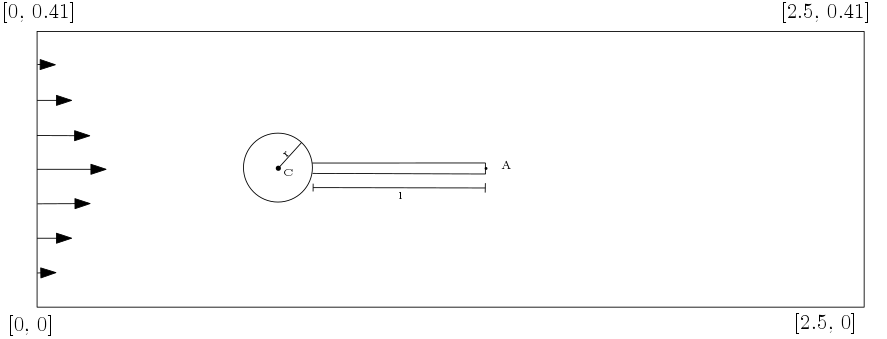
\includegraphics[scale=0.5]{./Fig/turekflag.png}
\end{figure}

Several quantites for comparion is presented in \cite{Hron2006} for validation purposes. We will report
\begin{itemize}
\item The position of point A(t) as the strucutre undergoes deformation.
\item Drag and lift forces exerted on of the whole interior geometry in contact with the fluid, consisting of the rigid circle and the elastic beam. 
\begin{align*}
(F_D, F_L) = \int_{\Gamma} \mathbf{\sigma} \cdot \mathbf{n} dS
\end{align*}
Where \textbf{n} is the unit normal vector, pointing into the fluid domain. 
\end{itemize}
The amplitude and mean values for the time dependent properties are calculated from the last period of oscillations, together with the period. 

\begin{table}[h]
\centering
\caption{Benchmark environment}
\label{my-label}
\begin{tabular}{ |p{3cm}||p{3cm}|p{3cm}|p{3cm}|  }
 \hline
 \multicolumn{4}{|c|}{Solid parameters} \\
 \hline
 parameter              & FSI1 & FSI2 & FSI3 \\
 \hline
 $\rho^s [10^{3} \frac{kg}{m^3}]$ & 1    & 10   & 1    \\
$\nu^s$ & 0.4  & 0.4  & 0.4  \\
$\mu^s  [10^{6}\frac{kg}{ms^2}]$  & 0.5  & 0.5  & 2.0  \\
 \hline
 \multicolumn{4}{|c|}{Fluid parameters} \\
 \hline
$\rho^f [10^{3}\frac{kg}{m^3}]$ & 1    & 1    & 1    \\
$\nu^f  [10^{-3}\frac{m^2}{s}]$  & 1    & 1    & 1    \\
U                      & 0.2  & 1    & 2    \\
parameter              & FSI1 & FSI2 & FSI3 \\
Re                     & 20   & 100  & 200 \\
\hline
\end{tabular}
\end{table}


\subsection{FSI1}
The first environment yields a steady state solution for the system. It is meant as a basic implementation test as it applies small deformations to the system. Therefore is provides a test for the solving procedure, but doesn't excess large constrain of choice of mesh extrapolation operator. 

\begin{table}[h!]
\centering
\caption{FSI 1}
\label{my-label}
\begin{tabular}{ |p{2.5cm}||p{1cm}|p{1cm}|p{2.3cm}|p{2.3cm}|p{1.2cm}|p{1.2cm}|}
 \hline
  \multicolumn{7}{|c|}{$\Delta t = 0.5$} \\
   \hline
 Model & nel & ndof & ux of A [x $10^{3}$]  &uy of A [x $10^{3}$]& Drag  & Lift \\
 \hline
Biharmonic bc2 & 1 &1 & 0.0228  &  0.7740  & 14.17280  &  0.7614 \\
 \hline
Biharmonic bc1 & 1 &1 & 0.0228 &   0.7737  & 14.17281 &  0.7612  \\
 \hline
Elastic        & 1 &1 & 0.0227  &  0.7960  & 14.17283 &  0.7607  \\
 \hline
Laplace        & 1 &1 & 0.0227  &  0.7958  & 14.17285 &  0.7607   \\
 \hline
  \multicolumn{7}{|c|}{$\Delta t = 0.1$} \\
   \hline
 Model & nel & ndof & ux of A [x $10^{3}$]  &uy of A [x $10^{3}$]& Drag  & Lift \\
 \hline
Biharmonic bc2 & 1 &1 & 0.0228 &  0.7743  & 14.17279 & 0.76162  \\
 \hline
Biharmonic bc1 & 1 &1 & 0.0228  &  0.7739 & 14.17280 & 0.76142 \\
 \hline
Elastic       & 1 &1 & 0.0228  &  0.7962  & 14.17281 & 0.76092 \\
 \hline
Laplace        & 1 &1 & 0.0228  & 0.7961  & 14.17284 & 0.76090 \\
\hline
\end{tabular}
\end{table}

\subsection{FSI2}
The second environment results in a periodic solution. It proved to be one of the most demanding tests due to its large deformation, leading to the risk of entangled mesh cells. As such this raised the need for a high quality extrapolation of the solid deformation.
\\
\subsection{FSI3}    
The final environment does not induce deformation to the extent of the FSI2 benchmark. However a critical phase in the transition to the periodic solution was discovered, where the pressure oscillation induces a large deformation to the system. 

\begin{table}[h!]
\centering
\caption{FSI 3}
\label{my-label}
\begin{tabular}{lllll}
 \hline
Test & x-comp A          & y-comp A             & drag                   & lift                 \\
 \hline
bc1 &                   &                      & 442.9 +/ 17.26         & 2.83 +- 148.8        \\
 \hline
bc2 &                   &                      & 442.8 +/ 17.44         & 3.06 +-147.9         \\
 \hline
Ref & 2.69  2.53  &   1.48  34.38 5.3   & 457. 22.66 10.9 & 2.22 149.78 5.3 \\
 \hline
\end{tabular}
\end{table}


\section{Mesh movement}
The final enviroment 
%\newpage

%\chapter{Application}
\section{Numericnerding eller applik ?}


\bibliographystyle{plain}
\bibliography{./Cite/Books,./Cite/ALECoupled,./Cite/Decoupled,./Cite/NavierStokes,./Cite/Verification,./Cite/EulerianFormulation,./Cite/Meshupdate}
\end{document}  
